%=========================================================================
% fig-opts-copy-ex.tex
%=========================================================================

\begin{figure}[b]

  \centering
  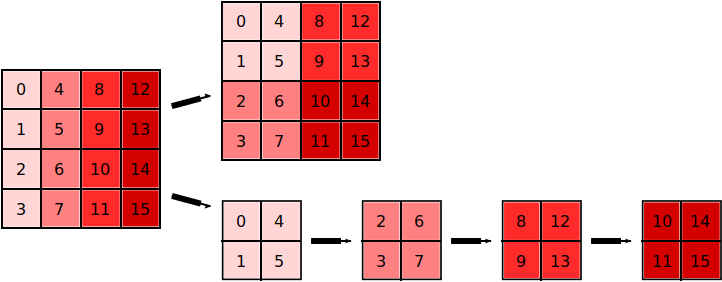
\includegraphics[width=0.9\tw]{fig-opts-copy-ex.svg.pdf}

  \caption{\textbf{Two Approaches to Copy Optimization --} The matrix on
    the left is arranged in column-major order in memory. It can be
    copied into a large scratchpad capable of storing all blocks (top
    path), or copied into a smaller scratchpad with enough space for one
    block (bottom path). In either case the data in each block is
    arranged to be contiguous in memory. The indices represent the data
    element in the original matrix and the colors represent contiguous
    segments in memory, with darker colors representing increasing
    addresses in memory.}

  \label{fig-opts-copy-ex}

\end{figure}
